%%%%%%%%%%%%%%%%%%%%%%%%%%%%%%%%%%%%%%%%%%%%%%%%%%%%%%%%%%%%%%%%%%%%%%
%%                     Logic arc
%%%%%%%%%%%%%%%%%%%%%%%%%%%%%%%%%%%%%%%%%%%%%%%%%%%%%%%%%%%%%%%%%%%%%%
%\color{blue}
\subsection{Glyph: \glyph{Logic arc} }\label{sec:logicArc}

\glyph{Logic arc} is the arc used to represent the fact that an entity influences
outcome of logic operator. 

\begin{glyphDescription}
 \item[SBO]\mbox{}\\ To be determined.
 \item[origin]\mbox{}\\ Any EPN (section \ref{sec:EPNs}) or logical operator (section~\ref{sec:logic}).
 \item[target]\mbox{}\\ Any logical operator (section~\ref{sec:logic}).
 \item[end-points]\mbox{}\\ No particular symbol is used to represent a source.
 \end{glyphDescription}

\begin{figure}[H]
  \centering
  \includegraphics[scale = 0.5]{images/logicArc}
  \caption{The \PD glyph for \glyph{logic arc}.}
  \label{fig:logicArc}
\end{figure}
